\renewcommand{\thechapter}{\Roman{chapter}}
\chapter{Review of Related Literature}
\renewcommand{\thechapter}{\arabic{chapter}}
\label{ch:rrl}
\thispagestyle{empty}

In this chapter, the researcher discussed the general idea of the volume estimation and filtering method and its several related studies. The chapter also presented some published and unpublished methods and technologies used for measuring the level and volume of the materials inside the silo (or sometimes called bin). 

Several traditional level measurements are already used and studied in different industries such as weight and cable methods, ultrasonic, Guided Ware Radar (GWR), and Thru-air Radar (TAR) which has their own advantage and disadvantages. Ultrasonic and laser technologies are excellent in providing accurate and detailed measurement of level. However, these technologies are problematic when in terms of dusty environment \citep{duysak2020}.

\section{3D Point Cloud Acquisition}
\label{rrl:sec:3D Point Cloud acquisition}
The recent advancements in spatial acquisition technologies such as aerial or terrestrial laser scanning have resulted in the formation of point clouds that may contain millions, billions, or trillions of points \citep{jaboyedoff2012}. Various 3D scanning technology produces data that are formatted as point cloud, typically these point cloud data acquired using laser or image scanner. These gathered data can be managed to ease the measurement and visualization of an object or environment \citep{chua2017}. Point cloud data are processed to generate desired output on the specific application. Over the past 20 years, the advent of high-quality 3D point cloud acquisition changes the perspective of robotics. Moreover, 3D scanning through various technologies enable the possibility of less contact for physical measurement that eliminate the traditional approach that involves time and effort. Unfortunately, most of these 3D sensors are expensive and therefore various relevant projects are considering not to use these sensors and opt to utilize alternative technology \citep{rusu2011}. 

\subsection{Light Detection and Ranging (LiDAR)}
\label{rrl:subsec:Light Detection and Ranging}
LiDAR is a remote sensing technology that uses laser light to create precise 2D or 3D models of objects or environments. LiDAR systems emit laser pulses that bounce back from objects in the environment, and the time taken for the light to return is used to determine the distance between the object and the sensor which called Time-of-Flight (ToF). By combining the distance measurements from multiple laser pulses, a point cloud can be generated that represents the shape and structure of the objects in the environment, Figure \ref{fig:Typical LiDAR System} shows the block diagram of a typical LiDAR system. LiDAR technology have been used in industrial settings. In the context of LiDAR scanning, individual point cloud scans are acquired and processed for a specific area. These point clouds are then merged and blended together to generate a complete point cloud of the desired area, which can be utilized for distance and measurement calculations \citep{jaboyedoff2012, raj2020}.

A 360-degree scan of a LiDAR is generally obtained in figure \ref{fig:360-dgree-lidar-scan} to produce a 2D map, a typical scan using the robot's top-mounted 2D LIDAR. The axis of the rotating LIDAR sensor is shown as a red line. The border of the surrounding obstacles is indicated in blue \citep{sarker2020}.

\begin{figure}[H]
    \centering
    \begin{minipage}{0.5\textwidth}
        \centering
        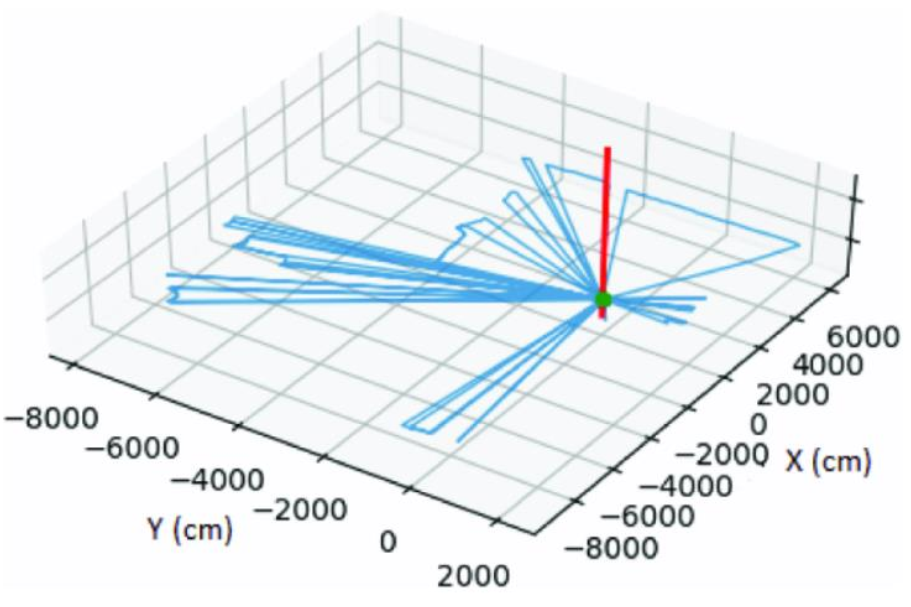
\includegraphics[width=0.9\textwidth]{Figures/360-degree-lidar-scan.png} % first figure itself
        \caption{360-degree scan of 2D LiDAR}
        \label{fig:360-dgree-lidar-scan}
    \end{minipage}\hfill
    \begin{minipage}{0.5\textwidth}
        \centering
        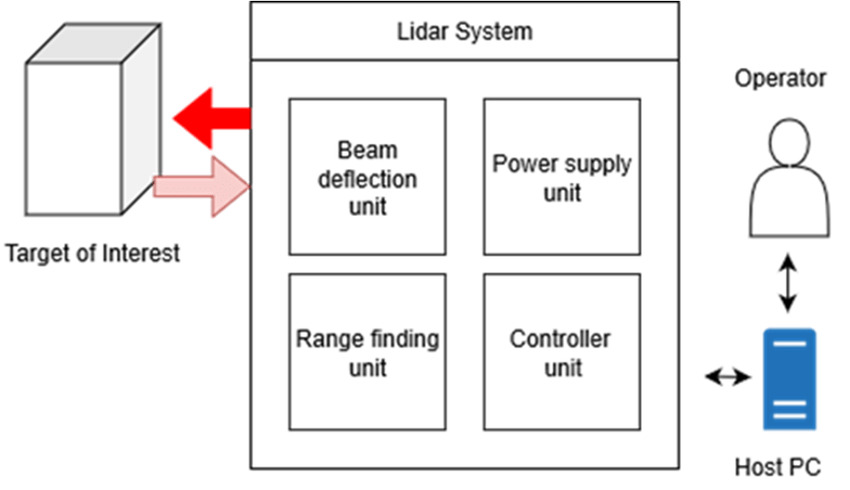
\includegraphics[width=0.9\textwidth]{Figures/Block-diagram-of-light-detection-and-ranging-LiDAR-system} % second figure itself
        \caption{Typical LiDAR System}
        \label{fig:Typical LiDAR System}
    \end{minipage}
\end{figure}

\citet{kang2018} utilized a 2D low-cost off-the-shelf LiDAR to reconstruct complex 3D model by integrating an external rotary for additional dimension. The experimental test achieved to evaluate 3D reconstruction by concluding that using a low-cost 2D LiDAR sensors can  perform 3D point cloud acquisition but increase either the complexity of its hardware or software. Figure \ref{fig:The principle of moving 2D LiDAR} illustrate the principle of 3D concept based on moving 2D LiDAR with 2 fixed different position in a room, the world coordinate frame is denote as 
\begin{math}
    W-X_{W}Y_{W}Z_{W}.
\end{math}
Although moving 2D LiDAR can never replace commercial 3D LiDAR with several reasons especially with applications involving real-time performance, however, moving 2D LiDAR can be partially used and installed with in terms of static and nonmoving environment \citep{bi2021}.

\begin{figure}[H]
    \centering
    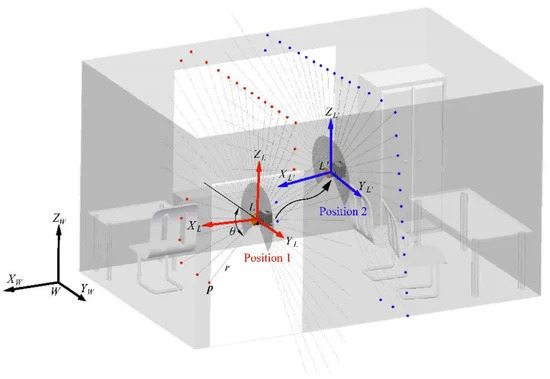
\includegraphics[width=0.7\textwidth]{Figures/moving-2D-LiDAR-principle.jpg}
    \caption{The principle of moving 2D LiDAR}
    \label{fig:The principle of moving 2D LiDAR}
\end{figure}

\section{Point Cloud Processing}
\label{rrl:sec:Point Cloud Processing}
Recent advancements in 3D reconstruction and visualization based on point cloud data have led to rapid development in various fields due to the rich data information and detailed real-world representation of objects or environments. Consequently, this massive data, including enormous kinds of noise, is overwhelmingly tedious to manage \citep{li2020}.

In the study conducted by \citet{wang2020}, when point cloud data are involved in construction applications, different point cloud data processing procedures are crucial to achieving desired outputs. Figure \ref{fig:data-processing} shows the common procedures for the raw point cloud data in a construction setting \citep{wang2020}.

\begin{figure}[H]
    \centering
    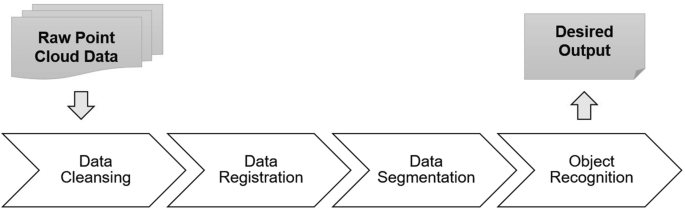
\includegraphics[width=0.9\textwidth]{data-processing}
    \caption{Typical processing procedures of point cloud data}
    \label{fig:data-processing}
\end{figure}

\citet{stanislas2021} divided the point cloud processing into four-step processes, figure \ref{fig:The-four-stages-of-the-point-cloud-classification-process} illustrates the structure of the authors, the point cloud output of the method is the same point cloud that was inputted before the classification took place. The method involves feature computing, data formatting, network prediction, and post-processing.

\begin{figure}[H]
    \centering
    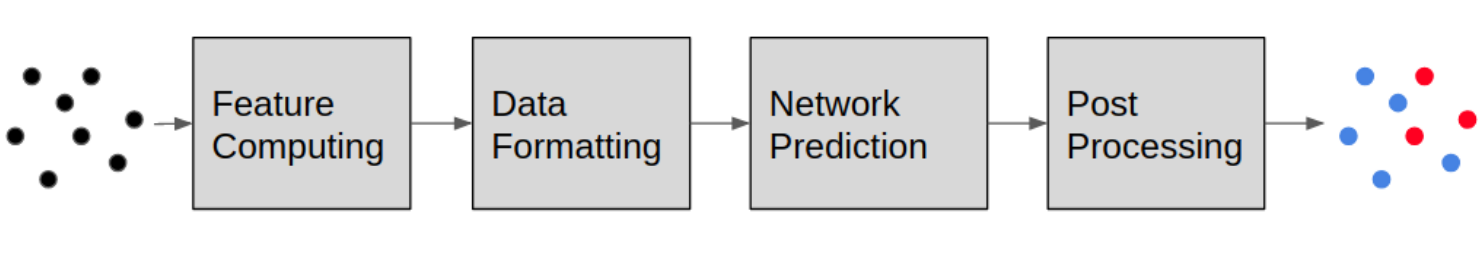
\includegraphics[width=\textwidth]{Figures/four-stage-of-pc-classification-process.png}
    \caption{The four stages of the point cloud classification process}
    \label{fig:The-four-stages-of-the-point-cloud-classification-process}
\end{figure}

\subsection{Outlier Point Cloud Processing}
\label{sub:Point Cloud Processing}
Processing of point cloud data by filtering is intensively exposed in research with a wide variety of applications. Cleaning of raw 3D point clouds is commonly the first step for most geometry processing, it involves removing the outliers (e.g., dust, snow, fog, etc.) after classifying the dust and non-dust (inliers) point cloud, smoothing the remaining data, and then reconstructing the surface into a three-dimensional representation \citep{rakotosaona2020}. Artificial Intelligence techniques such as Machine Learning (ML) and Deep Learning (DL) are widely used in classifying point cloud dust and non-dust data to remove noise.

For instance, \citet{stanislas2018} detected dusty regions in point cloud data by using machine learning techniques as well as specialized neural networks. The 3D map was transformed into 3D occupancy grids in this investigation, and the occupied voxels were utilized to train classifiers based on machine learning to extract significant information, figure \ref{fig:pcl seg} shows the result of the study.

\begin{figure}[H]
    \centering
    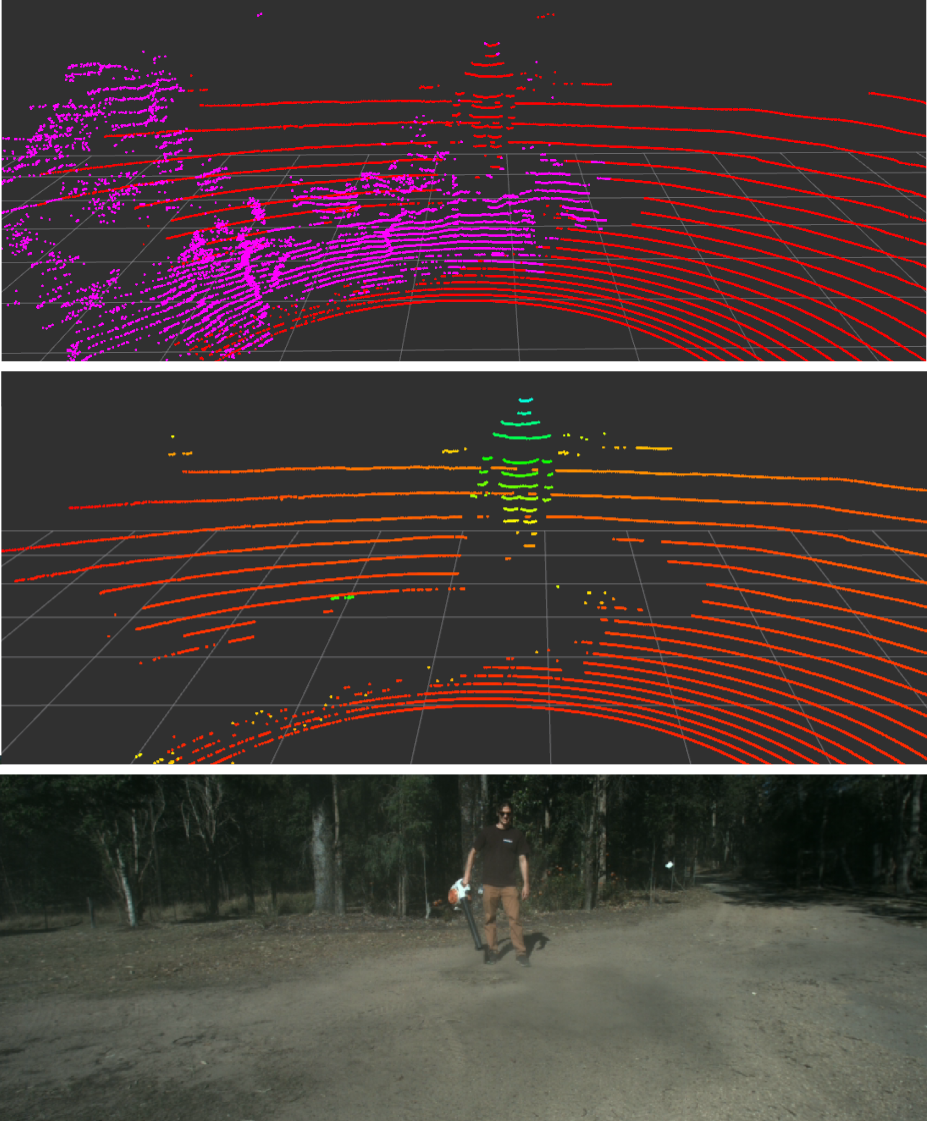
\includegraphics[width=0.7\textwidth]{pcl_seg}
    \caption{Top: Detection of airborne dust particle in a LiDAR point cloud, purple is Particle and red is Non-particle. Middle: Removal of detected dust particles from point cloud for robust perception, the color is mapped to the vertical axis (red is low, green is high). Bottom: Image depicting the scene.}
    \label{fig:pcl seg}
\end{figure}

The same voxel-based approach was also used in the study of \citet{shamsudin2016} for the classification of fog. The method involved using geometrical features and intensity as inputs for the support vector machine (SVM) and k-nearest neighbors (KNN) algorithms to classify fog.

Both point- and voxel-based categorization were taken into account in study by \citet{stanislas2021}. They experimented with various classifier input features to determine the most effective one for dust removal in order to boost performance. These characteristics include geometry, intensity, and multi-echo data from the LiDAR sensor. With point-based deep learning techniques, geometry, and multi-echo features proved to be the most useful features, while voxel-based deep learning techniques benefited from the addition of intensity information to these features.

To simplify the point cloud models and reduce the noise in point cloud data, \citet{zhu2020} employed the point-based simplification and guided filter. The guided filter was employed to filter the noisy point cloud model and generate the filtered image. The surface-based filtering group employs the filtering algorithm.

\citet{ramiya2017} set a threshold by measuring the distance between every point and the mean surface. They assigned a weight to each point based on its distance from the interpolated mean surface.

\citet{heinzler2020} used a large point cloud data set for CNN-based approach segmentation in controlled adverse weather effects. The approach takes a global understanding of the scene to estimate the validity of individual point measurements, rather than analyzing local spatial statistics as in previous approaches, it also proposes data augmentation technique that reduces the necessity for annotated ground truth data.

The multi-echos and intensity data features of LiDAR point cloud are utilized in various studies. \citet{afzalaghaeinaeini2021} used low-intensity outlier removal (LIOR) filtering for de-dusting method. The method is composed of two procedures: First, dust particles based on point cloud usually have a lower intensity compared to non-dust point cloud, point cloud with an intensity lower than the set threshold are removed. Second,  the study successfully filtered the point cloud data and removed the dust from the original point cloud data. 

Intensity-based filter was also utilized by \citet{park2020} for removal of snow in point cloud data. The study concluded that this method overcomes the disadvantages of LiDAR sensor compared to other conventional filtering methods.

\subsection{3D Space Point Cloud Mapping}

In todays generation, various point cloud processing and mapping frameworks are widely available to lessen the complexity of handling raw point cloud data, such as, Robotic Operating System (ROS), Point Cloud Library (PCL), Open3D, MeshLab, etc. Most of this framework can be used in many different fields such as virtual reality, construction, industry, and surveying.

The PCL has a built-in visualization library that uses Visualization ToolKit (VTK) as its foundation. VTK is a versatile platform that can render 3D point clouds and surfaces, and supports visualizing tensors, textures, and volumetric methods. The PCL Visualization library aims to merge PCL with VTK by providing a complete visualization layer for n-D point cloud structures. Its main goal is to allow for rapid prototyping and visualization of algorithm results on high-dimensional data \citep{rusu2011}.

\citet{ocando2017} take advantage of using ROS framework to map the 3D point cloud data, as the framework allows to interlink programs that is written in different languages. The study successfully addressed the problematic tasks of Simultaneous Localization and Mapping (SLAM) and 3D Octomapping via single sensor.

\section{Volume Estimation}
\label{rrl:sec:Industrial Volume Measurement}
Typically in an agriculture and food company setting, calculating the volume of a storage bin involves determining both the storage geometry and the distance between the grain surface and the eave. Traditionally, a fiberglass tape measure with weights is used to calculate the distance between the surface of the grain and the top of the bin. Correction factors are applied to the measurement to account for any irregularities in the surface of the grain, such as when the surface is uneven or when there is a cone-shaped pile \citep{turner2016}. These correction factors are usually simple to apply when the surface is relatively flat and equal in height. Moreover, these traditional approaches necessitate such effort and involved the employees to be at the top of the bin during the estimation. New methods and technologies have been trying to incorporate in industrial settings to eliminate these traditional methods such as using Microwaves Radar \citep{vogt2017}, Horn Antennas-based \citep{duysak2020, yigit2015}, Load Cell, Ultrasonic, Laser-based \citep{geuvara2020}, and Temperature-based sensor \citep{rhee2021}. Each of this technology has their own advantage and disadvantages, however, laser-based sensor (e.g. LiDAR) shows an interesting capabilities and features especially in acquiring three-dimensional point cloud data that can be used for geometric computation and for 3D object representation.

Point clouds in 3D are highly valuable as they contain crucial information on the shape, size, area, and volume of objects. Various industries, including agriculture and fisheries, have effectively utilized volume estimating methods based on point clouds \citep{geuvara2020}.

In computer graphics, a voxel is an image that depicts a specific region that has been partitioned into a grid of cubes that are all the same size and uniformly spaced \citep{putman2018}.

Due to a better portrayal of the region encompassed in the group of points, the Delaunay triangulation and voxelization procedures outperform in estimating the outcomes. These strategies, however, have a greater computational cost because of their accuracy \citep{chee2015}. To estimate volume, methods such as Delaunay triangulation and voxelization are used. It is important to consider both accuracy and computing costs when using these methods. Height grids are faster for computing height discrepancies, but accuracy depends on precise point acquisition \citep{bewley2011, duff2000}.

The Delaunay triangulation-based technique for volume computation, known as Delaunay triangulation-driven volume calculation (DTVC), differs from traditional approaches which computes the volume during the triangulation process rather than preserving Delaunay triangles. This method reduces both memory usage and processing time. Experimental findings demonstrate that DTVC achieves a satisfactory trade-off between precision and efficiency \citep{liuY2021}.

Table \ref{tab:Point Cloud Volume of Different Objects} shows the percentage error analysis from the computed volume of different model point cloud objects in the study of \citet{chang2017}, which shows that in order to estimate the volume of a shape represented by a point cloud, the area of each slice of the shape is calculated by finding the difference between the top and bottom curves of the slice. The total volume of the shape is then calculated by integrating the areas of all the slices using an integration interval equal to the length of the point cloud. 

\begin{table}[H]
\caption{Point Cloud Volume of Different Model}
\label{tab:Point Cloud Volume of Different Objects}
\centering
\begin{tabular}{|c|c|c|c|}
    \hline
    % First row
    Objects & True Value (\si{mm^3}) & Estimated Value (\si{mm^3}) & Error (\%) \\
    \hline
    % Second row
    Cube &  1 000 000 & 1 000 000 & 0 \\
    \hline
    % Third row
    Cylinder & 125.664 & 125.061 & 0.479 \\
    \hline
    % Fourth row
    Sphere & 4 188 90.2 & 4 178 966.87 & 0.234 \\
    \hline
    % Fifth row
    Triangle Prism & 17.321 & 17.399 & 0.45 \\
    \hline
\end{tabular}
\end{table}

The study conducted by \citet{jeong2018} introduces a newly developed explicit hybrid numerical methodology for 3D volume reconstruction from unorganized point clouds, which is based on a modified Allen-Cahn equation and a 3D binary picture segmentation method. The technique has demonstrated potential in a variety of practical applications, including 3D model printing from dispersed scanned data. The computational findings show that the suggested approach for reconstructing 3D volume from point clouds is very efficient and resilient.

The Convex Hull is another method that is popular technique for measuring volume from 3D point cloud points (see figure \ref{fig:convex hull}). The computational geometry community has extensively studied the convex hull problem, as evidenced by the works of \citet{kim2002}, \citet{graham1983}, and \citet{maus1984}. Qhull is a commonly used algorithm to compute the convex hull, employing the Voronoi diagram, the Delaunay triangulation, furthest-site Voronoi diagram, the furthest-site Delauney triangulation, and the half-space intersection around a point. The software program allows the creation of high-dimensional objects, and the Quickhull algorithm, written in C, is used to compute the convex hull, which solves round-off errors in floating-point arithmetic. The program is capable of calculating volumes, surface areas, and convex hull approximations.

\begin{figure}[H]
    \centering
    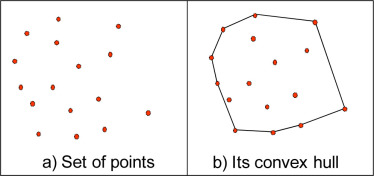
\includegraphics[width=0.8\textwidth]{Figures/convex hull.jpg}
    \caption{Convex Hull}
    \label{fig:convex hull}
\end{figure}

\section{Synthesis of the Study}

The review of related literature conducted and summarized by the researcher are pertinent to guide the researcher in order to achieve the objectives of the study. The review identifies the need for different point cloud data processing procedures to achieve desired outputs. The review also highlights various point cloud processing techniques such as, machine learning (ML), and deep learning (DL) techniques for removing noise and classifying point cloud dust and non-dust data, however, the challenges of these AI approaches with point cloud data for filtering is the amount of data that will be stored for the training method which necessitate millions of point clouds. Another is the high computational cost of these training methods. Lastly, the performance of the method is significantly dependent on its datasets. 

While several studies have explored the use of various classifier input features to remove noise, the most effective features have been found to be geometry, intensity, and multi-echo data from the LiDAR sensor. However, there is a gap in the study regarding the evaluation of the performance of these techniques in real-world applications. The need for further research with regard to these methods in a real-world scenarios is highly significant. Thus, this study will address the gap mentioned by integrating these techniques into a real-world applications and identify their practical implications.